% CEII 2026 (9th Asia Conference on Cognitive Engineering and Intelligent Interaction) -- proceedings in Springer
% "Lecture Notes in Networks and Systems". Springer LLNCS class (llncs.cls v2.24) and splncs04.bst from the
% conference's LaTeX template package. Full papers: 8-10 pages including figures, tables and references.
\documentclass[runningheads]{llncs}
\usepackage[T1]{fontenc}
\usepackage{amsmath,amssymb}
\usepackage{graphicx}
\usepackage{booktabs}
\usepackage{multirow}
\usepackage{cite}
\usepackage{marvosym} % \Letter marks the corresponding author
\usepackage[hidelinks]{hyperref}
\usepackage{color}
\renewcommand\UrlFont{\color{blue}\rmfamily}
\urlstyle{rm}

\newcommand{\FDRb}{\mathrm{FDR}_{\mathrm{b}}}
\newcommand{\FDRp}{\mathrm{FDR}_{\mathrm{pool}}}

\begin{document}

\title{Guaranteed versus Experienced False-Alert Rates: A Pre-registered Evaluation of Conformal Selection for Provincial Dengue Outbreak Bulletins}
\titlerunning{Guaranteed versus Experienced False-Alert Rates}

\author{Van Quang Tran\inst{1,2} \and
Vo Dinh Kha Le\inst{1,2}\textsuperscript{(\Letter)}}
\authorrunning{V. Q. Tran and V. D. K. Le}

\institute{University of Information Technology, Ho Chi Minh City, Vietnam \and
Vietnam National University, Ho Chi Minh City (VNU-HCM), Ho Chi Minh City, Vietnam\\
\email{quangtv.20@grad.uit.edu.vn, khalvd@uit.edu.vn}}

\maketitle

\begin{abstract}
Dengue early-warning systems issue a monthly bulletin that lists the provinces expected to exceed an epidemic threshold, and they are trusted only if few of those alerts are false. Conformal selection, which applies the Benjamini--Hochberg (BH) procedure to conformal p-values, can promise in advance that the expected share of false alerts \emph{per bulletin} stays below a level $q$. A health officer, however, experiences the share of false alerts among \emph{all} alerts received, which is a different quantity. We measure this difference on real surveillance data in a pre-registered design: monthly counts for 337 provinces in nine countries, probabilistic forecasts 1--3 months ahead, five development countries and four held-out confirmation countries (the Philippines, Viet Nam, Sri Lanka and Brazil). At $q=0.2$, the guarantee holds (bulletin false discovery rate 0.12--0.13), but the false-alert share users receive is 0.225, 0.277 and 0.332 at 1, 2 and 3 months ahead. This gap is 0.09--0.17 larger than that of a simple fixed-threshold rule, and the result survives burn-in exclusion and the removal of any single country. On the experienced scale the fixed-threshold rule dominates conformal selection at every horizon, whereas on the guaranteed scale conformal selection has higher recall at 2--3 months. About 40--57\% of the gap comes from forecast errors shared by the provinces of the same month. Neither an epidemic-state (Mondrian) calibration nor Learn-then-Test certification closes the gap. Agencies should therefore decide which false-alert rate a bulletin promises before choosing the alerting rule.

\keywords{Conformal Selection \and False Discovery Rate \and Early Warning System \and Dengue \and Outbreak Detection \and Pre-registration}
\end{abstract}

% =====================================================================
\section{Introduction}

\subsection{Motivation}
Dengue is the fastest-spreading mosquito-borne viral disease, and South and South-East Asia carry most of its burden. Provincial health departments must decide one to three months in advance where to spray, where to stock intravenous fluids and where to open surge beds. Early-warning systems support these decisions with a bulletin that flags the provinces expected to exceed an endemic threshold \cite{bortman1999,hussain2018ewars,lowe2016}. A bulletin is useful only if people trust it, and they trust it only if it is rarely wrong, because every false alarm costs vector-control resources and credibility.

\subsection{Problem Statement and Research Gap}
Conformal selection \cite{jin2023selection} offers a finite-sample promise of the kind an agency would like to announce: ``on average, at most 20\% of the flagged provinces will be false alarms''. The false discovery rate (FDR) in that sentence is $\mathbb{E}[V/\max(R,1)]$ over bulletins, where $V$ is the number of false alerts and $R$ the number of alerts in one bulletin; a bulletin without alerts contributes zero. A health officer instead experiences the share of false alerts among all alerts received over a season, $\sum V/\sum R$, which is the marginal FDR \cite{genovese2002,sun2007}. The two notions are classical, and the theory predicts that they can differ. Three things are still missing: (i) a measurement of how large the difference is on real multi-country surveillance data; (ii) a test of whether it changes which alerting rule an agency should prefer; and (iii) an explanation of where it comes from. Existing dengue warning systems report sensitivity and positive predictive value at fixed thresholds and make no announced error-rate promise \cite{lowe2016,hussain2018ewars}, while the conformal literature evaluates its guarantee on the quantity it controls.

\subsection{Research Questions and Hypotheses}
This study answers three research questions (RQ) and tests five pre-registered hypotheses (H), all at $q=0.2$:
\begin{itemize}
\item \textbf{RQ1.} Does conformal selection keep its per-bulletin guarantee on held-out countries, and how far is the experienced (pooled) FDR from it? \textbf{(H1)} The upper 95\% CI of the bulletin FDR is at most $q$ at every horizon. \textbf{(H2)} The gap $\Delta=\FDRp-\FDRb$ has a lower CI above 0 at every horizon. \textbf{(H2b)} The gap of conformal selection exceeds that of a pre-specified fixed-threshold rule.
\item \textbf{RQ2.} Which rule is preferable on the experienced scale? \textbf{(H4)} Conformal selection is dominated on (pooled FDR, recall) by a member of a fixed-threshold family at two or more horizons.
\item \textbf{RQ3.} Can the gap be reduced or labelled? \textbf{(H3)} An epidemic-state Mondrian calibration lowers the pooled FDR. \textbf{(H5)} A trailing-precision label meets its 90\% bound in at least 85\% of country-years.
\end{itemize}

\subsection{Contributions}
The contributions of this work are:
\begin{description}
\item[C1] A pre-registered\footnote{Code, data sources, the frozen pre-registration and all result files are available at [repository URL].} evaluation of conformal selection for multi-province outbreak bulletins on nine countries, with a development/confirmation split by country and a fixed mapping from outcomes to claims.
\item[C2] A quantified gap between the guaranteed and the experienced FDR, with paired, country-stratified confidence intervals and an exact decomposition into an empty-bulletin part and an alert-weighting part.
\item[C3] An attribution of the gap to forecast errors shared within a month, by a data-based permutation reference and a simulation calibrated to the observed error structure.
\item[C4] Transparent negative results (Mondrian calibration, Learn-then-Test certification and trailing-precision labels) and a reporting protocol for health agencies.
\end{description}

% =====================================================================
\section{Related Work}

\subsection{Background}
The BH procedure \cite{benjamini1995} controls $\mathbb{E}[V/\max(R,1)]$ under independence and positive dependence \cite{benjamini2001}. When $R$ is random, this differs from the positive FDR $\mathbb{E}[V/R\mid R>0]$ \cite{storey2003} and from the marginal FDR $\mathbb{E}[V]/\mathbb{E}[R]$ \cite{genovese2002}; for the marginal FDR the optimal rule is a single global threshold on a local-fdr statistic \cite{sun2007}. Conformal p-values \cite{vovk2005,bates2023} compare a new score with the scores of past cases and need no distributional assumption. Combined with BH they select units whose outcome exceeds a threshold with finite-sample FDR control \cite{jin2023selection}. Extensions address non-exchangeable data \cite{barber2023,gibbs2021}, general risks \cite{angelopoulos2024crc,angelopoulos2021ltt} and sequences of selections \cite{javanmard2018,zrnic2020}.

\subsection{Prior Work and Limitations}
Dengue forecasting studies evaluate point or probabilistic accuracy \cite{johansson2019,colon2021vietnam,bracher2021}. Early-warning systems such as EWARS \cite{hussain2018ewars} and the Brazilian prototype \cite{lowe2016} turn forecasts into alerts with an endemic-channel threshold \cite{bortman1999}, but report detection skill without an announced false-alert promise. Conformal selection supplies such a promise, yet its evaluations report the guaranteed quantity. To our knowledge, no study has measured the guaranteed and the experienced FDR side by side on real outbreak bulletins, or asked whether the choice between them changes the recommended rule. The theory behind the two notions is classical; this study measures how large the difference is in practice and what it changes.

% =====================================================================
\section{Methodology}

\subsection{Overview}
The pipeline has four stages (Fig.~\ref{fig:pipeline}): monthly provincial counts, probabilistic forecasts taken from a companion study (seven quantiles, 1--3 months ahead), alerting rules that turn the forecasts into a monthly bulletin, and an evaluation of every rule on both FDR notions.

\begin{figure}[!htbp]
\centering
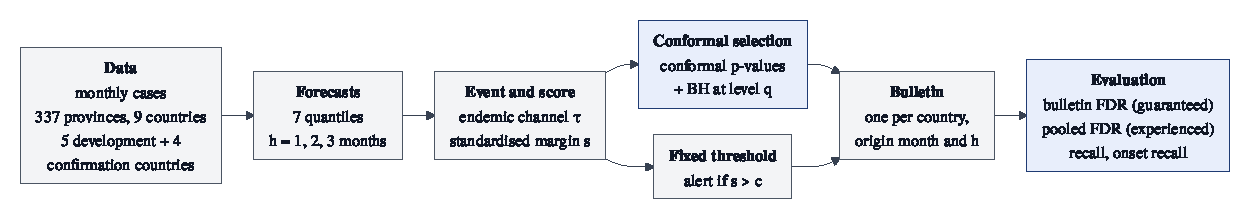
\includegraphics[width=\textwidth]{figures/fig_pipeline.pdf}
\caption{Pipeline of the study. Each alerting rule (conformal selection, the fixed-threshold family, and the CRC and top-$k$ baselines) issues one bulletin per country, origin month and horizon; every bulletin is scored on both FDR notions.}
\label{fig:pipeline}
\end{figure}

\subsection{Data and Data Pipeline}
Monthly dengue counts at the first sub-national level (province or state) come from OpenDengue V1.3 \cite{clarke2024opendengue} and national portals. The Viet Nam series (60 provinces, 1998--2010) was compiled by the authors from public sources; provinces that were split or merged were re-aggregated so that each forms one continuous series. Missing months are left missing (2.9\% of province-months in South-East Asia 2006--2010, 0.3\% in 2015--2024). Countries are split before any analysis into a development set, used to design the procedures, and a confirmation set, run once after the hypotheses were frozen (Table~\ref{tab:data}). The data are aggregated public counts with no identifiable information.

\begin{table}[!htbp]
\caption{Countries, roles and event rates}
\label{tab:data}
\centering
\setlength{\tabcolsep}{4pt}
\begin{tabular}{llrlr}
\toprule
Role & Country & Units & Test years & Event rate \\
\midrule
\multirow{5}{*}{Development} & Thailand & 77 & 2015--2022 & 16.0\% \\
 & Indonesia & 32 & 2015--2022 & 18.0\% \\
 & Cambodia & 24 & 2006--2010 & 16.3\% \\
 & Laos & 16 & 2006--2010 & 20.5\% \\
 & Malaysia & 10 & 2006--2010 & 24.8\% \\
\midrule
\multirow{4}{*}{Confirmation} & Philippines & 65 & 2006--2010 & 35.1\% \\
 & Viet Nam & 60 & 2006--2010 & 17.4\% \\
 & Sri Lanka & 26 & 2016--2024 & 23.6\% \\
 & Brazil & 27 & 2017--2024 & 17.4\% \\
\bottomrule
\end{tabular}
\end{table}

\textit{Event.} A province-month is an \emph{endemic-channel exceedance} when $\log(1+\text{cases})$ exceeds the mean plus two standard deviations of the same calendar month in the previous five years (highest year excluded), with at least five cases \cite{bortman1999}. An \emph{onset} is an event month whose previous month is not an event.

\textit{Forecasts.} On the confirmation set the forecasts are the companion study's ensemble: a per-quantile average, on the log scale, of a LightGBM model pooled across countries \cite{ke2017lightgbm} and the zero-shot foundation model Chronos-2 \cite{ansari2025chronos2}. LightGBM hyper-parameters are tuned only on years before each test year, and Chronos-2 is not trained. The risk score is a standardised margin,
\begin{equation}
s=\frac{\log(1+\hat q_{0.5})-\tau}{\max\{\log(1+\hat q_{0.9})-\log(1+\hat q_{0.1}),\,0.05\}},
\end{equation}
where $\tau$ is the log endemic threshold; a cell is \emph{eligible} if $\hat q_{0.5}\ge 5$ cases.

\subsection{Alerting Procedures}
A \emph{bulletin} is one (country, origin month, horizon $h$).

\textit{Conformal selection (CS).} At origin $t$ the calibration set holds the eligible cells of the same country and horizon whose target month is already observed, with at least 200 cells. For an eligible cell $j$ with score $s_j$,
\begin{equation}
p_j=\frac{1+\#\{i\le n:\ Y_i=0,\ s_i\ge s_j\}}{n+1},
\end{equation}
where $Y_i=0$ marks a past non-event; ineligible cells get $p_j=1$. Alerts are the BH selection at level $q$. If calibration and test cells are exchangeable given eligibility, and the bulletin's cells are independent given the calibration set, then $\mathbb{E}[V/\max(R,1)]\le q$ \cite{jin2023selection}. Shared forecast errors violate exactly this exchangeability, so we treat the assumption as the object of study.

\textit{Remedy.} \emph{Mondrian CS} restricts calibration to past cells with the same national epidemic state (at least 20\% of provinces above their channel at the origin). It was the single remedy pre-registered for confirmation. Learn-then-Test \cite{angelopoulos2021ltt} and adaptive level feedback \cite{gibbs2021} were tried on development data only.

\textit{Baselines.} A frozen fixed-threshold family alerts when $s>c$ (or a margin without standardisation exceeds $c$), with $c\in\{-0.3,\dots,0.5\}$; the pre-specified comparator is the margin rule with $c=0$, i.e.\ ``alert when the median forecast exceeds the threshold''. A conformal-risk-control-style scan (CRC) \cite{angelopoulos2024crc} and a top-$k$ rule are descriptive baselines.

\subsection{Evaluation Protocol}
For every rule we report three FDR notions over the $B$ bulletins: the guaranteed bulletin FDR, the FDR of bulletins that contain alerts, and the experienced (pooled) FDR,
\begin{align}
\FDRb &= \tfrac{1}{B}\textstyle\sum_b V_b/\max(R_b,1),\\
\mathrm{FDR}_{>0} &= \operatorname{mean}\{V_b/R_b : R_b>0\},\\
\FDRp &= \textstyle\sum_b V_b \,/\, \sum_b R_b,
\end{align}
together with recall of event months, onset recall and lead time. The gap $\Delta=\FDRp-\FDRb$ decomposes exactly as
\begin{equation}
\Delta=\underbrace{(\mathrm{FDR}_{>0}-\FDRb)}_{\text{empty bulletins}}+\underbrace{\frac{\mathrm{Cov}(R,\mathrm{FDP}\mid R>0)}{\mathbb{E}[R\mid R>0]}}_{\text{alert weighting}},
\end{equation}
where the second term is positive when large bulletins are more often wrong. Confidence intervals (95\%) come from a country-year block bootstrap (1{,}000 resamples), and comparisons between rules use paired resamples. A country-stratified bootstrap and leave-one-country-out estimates serve as robustness checks.

% =====================================================================
\section{Experimental Setup}

The hypotheses H1--H5 and an outcome-to-claim table were frozen in three versions on public GitHub branches before the confirmation set was analysed. The main disclosed deviation is that origins without enough calibration cells (32--40 of 317 bulletins per horizon) were scored as empty for CS, whereas the plan excluded them. We therefore report results both with and without these burn-in origins. The confirmation set yields 317 bulletins per horizon. A simulation (40 provinces, 14 years, 300 replicates) adds a forecast error $w$ shared by all cells of a bulletin. Its share of the error variance is set to the value measured on the confirmation forecasts: the between-bulletin share of log forecast-error variance is 0.23--0.28 on average (0.05--0.08 for Viet Nam and 0.42--0.54 for Sri Lanka).

% =====================================================================
\section{Results}

\subsection{Guarantee and Experienced FDR (RQ1)}
Table~\ref{tab:main} summarises the confirmation results at $q=0.2$. The guarantee holds: the bulletin FDR of CS is 0.119--0.126, with upper CIs of 0.158--0.161 (H1 supported). The experienced FDR is much higher: 0.225, 0.277 and 0.332 at $h=1,2,3$. The gap $\Delta$ is 0.100, 0.153 and 0.212, with lower CIs of 0.062, 0.095 and 0.140 (H2 supported). Measured against the announced level, the pooled FDR is indistinguishable from 0.2 at $h=1$ (CI 0.184--0.276) but exceeds it at $h=2$ and $h=3$.

\begin{table}[!htbp]
\caption{Confirmation results at $q=0.2$, pooled over the four held-out countries (95\% CIs from the country-stratified bootstrap). $\FDRb$: bulletin (guaranteed) FDR; $\FDRp$: pooled (experienced) FDR; Alert-wt.\ part: alert-weighting term of Eq.~(6).}
\label{tab:main}
\centering
\scriptsize
\setlength{\tabcolsep}{2.5pt}
\begin{tabular}{@{}p{1.55cm}ccccccc@{}}
\toprule
Rule & $h$ & $\FDRb$ & FDR$_{>0}$ & $\FDRp$ [CI] & Gap $\Delta$ [CI] & Alert-wt.\ part & Recall \\
\midrule
\multirow{3}{1.55cm}{Conformal selection (CS)} & 1 & 0.126 & 0.193 & 0.225 [0.184, 0.276] & 0.100 [0.065, 0.149] & 0.032 & 0.644 \\
 & 2 & 0.124 & 0.241 & 0.277 [0.212, 0.351] & 0.153 [0.095, 0.226] & 0.036 & 0.454 \\
 & 3 & 0.119 & 0.274 & 0.332 [0.245, 0.417] & 0.212 [0.140, 0.296] & 0.057 & 0.326 \\
\midrule
\multirow{3}{1.55cm}{Fixed threshold, $c=0$} & 1 & 0.162 & 0.193 & 0.168 [0.137, 0.212] & 0.006 [$-$0.022, 0.038] & $-$0.025 & 0.682 \\
 & 2 & 0.214 & 0.268 & 0.236 [0.188, 0.292] & 0.022 [$-$0.015, 0.066] & $-$0.032 & 0.526 \\
 & 3 & 0.236 & 0.305 & 0.283 [0.231, 0.346] & 0.047 [0.005, 0.096] & $-$0.022 & 0.395 \\
\midrule
\multirow{3}{1.55cm}{CS, random pseudo-bulletins} & 1 & 0.160 & 0.194 & 0.197 & 0.037 & 0.003 & 0.688 \\
 & 2 & 0.146 & 0.221 & 0.230 & 0.084 & 0.009 & 0.484 \\
 & 3 & 0.158 & 0.266 & 0.260 & 0.102 & $-$0.006 & 0.356 \\
\bottomrule
\end{tabular}
\end{table}

The gap is specific to per-bulletin BH. The fixed-threshold rule has an almost zero gap, so the paired difference $\Delta_{\text{CS}}-\Delta_{\text{threshold}}$ is 0.093 [0.066, 0.129], 0.131 [0.096, 0.170] and 0.165 [0.120, 0.220] (H2b supported). The difference stays positive when burn-in origins are excluded (lower CIs 0.055, 0.084, 0.104) and when any one country is left out (range 0.086--0.186). The alert-weighting term is positive for CS (0.032--0.057) and negative for the threshold rule: when CS issues many alerts in one month, those alerts are more often wrong.

\subsection{Which Rule Is Preferable (RQ2)}
Fig.~\ref{fig:frontier} traces each rule family across its tuning range. On the experienced scale (top row), the fixed-threshold family dominates CS at every horizon (H4 supported). Against the pre-specified comparator $c=0$, CS has a higher pooled FDR by 0.057 [0.028, 0.083], 0.041 [0.010, 0.070] and 0.048 [0.004, 0.091], with no gain in recall. At a matched pooled FDR, the threshold rule also detects more epidemic onsets (0.465, 0.401, 0.346 against 0.340, 0.234, 0.189). On the guaranteed scale (bottom row) the ranking reverses. At a matched bulletin FDR, CS has higher recall at $h=2$ (+0.115 [0.054, 0.159]) and $h=3$ (+0.125 [0.067, 0.173]), and ties at $h=1$; this comparison was added after confirmation and is exploratory. The reversal is what theory predicts: the bulletin FDR rewards alert-free months, which BH produces in quiet periods, whereas a single global threshold is the optimal form for the marginal FDR \cite{sun2007}.

\begin{figure}[!htbp]
\centering
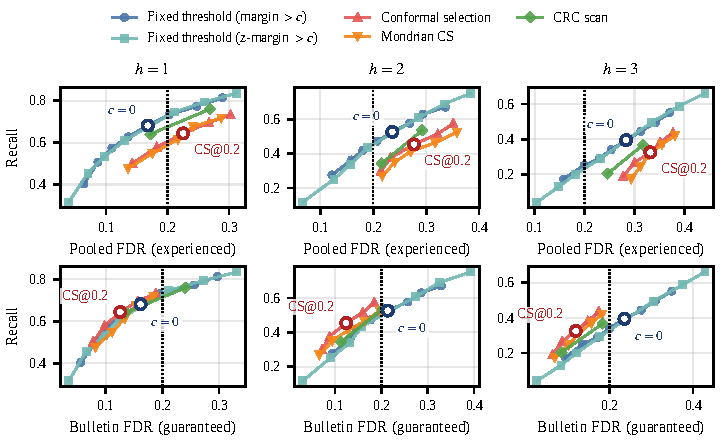
\includegraphics[width=\textwidth]{figures/frontier.pdf}
\caption{Precision--recall frontiers on the four confirmation countries. Top: experienced (pooled) FDR, where the fixed-threshold family dominates conformal selection. Bottom: guaranteed (bulletin) FDR, where conformal selection lies on or above the threshold frontier. Threshold curves trace $c$ from $-0.3$ to $0.5$; CS and Mondrian trace $q$ from 0.1 to 0.3. The dotted line marks $q=0.2$.}
\label{fig:frontier}
\end{figure}

\subsection{Where the Gap Comes From}
Regrouping the same conformal p-values into random pseudo-bulletins of the same sizes (within country, horizon and year) breaks the month-level grouping while keeping everything else. The gap then falls to 0.037, 0.084 and 0.102, and the alert-weighting term vanishes (Table~\ref{tab:main}). Compared with the burn-in-excluded gap (0.086, 0.137, 0.195), about 57\%, 39\% and 48\% of the gap is due to how alerts group into real months; the remainder is the classical difference that exists even under exchangeability. The simulation (Fig.~\ref{fig:sim}) shows the mechanism. Under i.i.d.\ errors CS is exact on its own quantity (0.204) yet already has a pooled FDR of 0.306. With the empirical shared-error share of 0.25, the gap of CS reaches 0.245, against 0.062 for the threshold rule, and it grows about 2.2 times faster with the shared error. The simulation illustrates the gap only, not the ranking of rules.

\begin{figure}[!htbp]
\centering
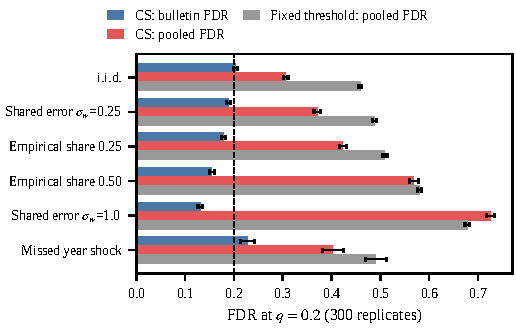
\includegraphics[width=0.68\textwidth]{figures/simulation.pdf}
\caption{Simulation at $q=0.2$ (bars: $\pm$1.96 Monte Carlo s.e.). The guaranteed FDR of CS stays near $q$, while its experienced FDR grows with the error shared within a bulletin.}
\label{fig:sim}
\end{figure}

\subsection{Remedies and Labels (RQ3)}
Mondrian calibration does not narrow the gap: its paired difference in pooled FDR from CS is $-0.008$ [$-0.025$, 0.010], $-0.006$ [$-0.037$, 0.022] and $-0.002$ [$-0.021$, 0.019] (H3 not supported). On the development set, Learn-then-Test with Hoeffding or empirical-Bernstein bounds issued at most 303 alerts out of several thousand eligible cells, and adaptive level feedback traded recall for precision. A trailing 24-month precision label met its 90\% lower bound in only 68--69\% of country-years (H5 not supported), because precision drifts between epidemic years.

% =====================================================================
\section{Discussion}

\textbf{H1 and H2 are supported:} conformal selection keeps its per-bulletin promise on held-out countries, yet the false-alert share that users receive is 0.10--0.21 higher. \textbf{H2b is supported:} the gap is a property of per-bulletin BH, not of alerting in general, since a fixed threshold has almost none. \textbf{H4 is supported:} on the experienced scale a simple threshold rule is the better operating choice, while on the guaranteed scale conformal selection is. \textbf{H3 and H5 are not supported:} at national data sizes neither the Mondrian state nor finite-sample certification recovers the experienced FDR, and a naive precision label is over-confident.

\textbf{Practical implications.} The choice of FDR notion decides the method. We recommend a short reporting protocol for agencies: (1) state in the bulletin whether the promise is per bulletin or per alert received; (2) when a conformal level is announced, also publish the realised pooled false-alert share and its year-to-year spread; (3) do not present a trailing-precision interval as a guarantee; and (4) compare any calibrated rule with a fixed threshold on the frontier of the chosen notion.

\textbf{Limitations.} The confirmation set has about 27 country-years, with only five test years for the Philippines and Viet Nam, so the intervals are wide; the stratified bootstrap and leave-one-country-out analysis lead to the same conclusions. The forecasts come from a single pipeline, the event is a statistical channel rather than a clinical threshold, and reporting delays are not modelled. Online and batch FDR procedures \cite{javanmard2018,zrnic2020} and betting-based bounds \cite{waudbysmith2024} were not evaluated.

% =====================================================================
\section{Conclusion and Future Work}
This study measured, on four held-out countries and under a pre-registered plan, the difference between the false-alert rate that conformal selection guarantees and the one that users of an outbreak bulletin experience. The guarantee held, but the experienced false-alert share was 0.09--0.17 further from it than under a fixed-threshold rule, and the threshold rule was preferable on the experienced scale. About half of the gap comes from forecast errors shared by the provinces of the same month. Alert systems should therefore state which false-alert rate they control, and should be evaluated on that rate's frontier. Future work includes online FDR procedures over the sequence of bulletins, external validation on other regions, and a monthly-updated warning dashboard for health agencies.


\begin{credits}
\subsubsection{\ackname} This research is funded by University of Information Technology - Vietnam National University Ho Chi Minh City under grant number [grant code].
% Springer policy: use of large language models is documented in the Methods section, not in the authorship;
% AI-assisted copy editing does not need to be declared.

\subsubsection{\discintname} The authors have no competing interests to declare that are relevant to the content of this article.
\end{credits}

\bibliographystyle{splncs04}
\bibliography{refs}

\end{document}
